\documentclass{article}
\usepackage{tikz}
\usetikzlibrary{arrows.meta, positioning, shapes.geometric}
\usepackage[utf8]{inputenc}
\usepackage[UTF8]{ctex}
\usepackage{pgfplots}
\pgfplotsset{compat=1.16}
\usetikzlibrary{calc}
\usepackage{amsmath}
\usepackage{amssymb}
\usepackage{array}
\usepackage{booktabs}
\usepackage{enumitem}
\usepackage{xeCJK}
\usepackage{CJKutf8}
\setCJKmainfont{Noto Serif CJK TC}    % 思源宋體繁體版(推薦)
\setCJKsansfont{Microsoft JhengHei}   % 微軟正黑體
\setCJKmonofont{Noto Sans Mono CJK TC}
% \setCJKmainfont{WenQuanYi Zen Hei}
% % 或者使用其他可用字體:
% % \setCJKmainfont{AR PL Mingti2L Big5}
% % \setCJKmainfont{Noto Sans CJK TC}

% % 設置全形符號支持
% \setCJKsansfont{WenQuanYi Zen Hei}
% \setCJKmonofont{WenQuanYi Zen Hei}

\title{Self-Injection-Locked (SIL) Oscillator Analysis}
\author{carlos ma}
\date{\today}
\usepackage[margin=1in]{geometry}
% \usepackage{tikz}
\usetikzlibrary{arrows.meta,positioning}
\usepackage{caption}
\begin{document}
\maketitle

% \section{QSIL}
\section*{Unwrap 的概念與必要性}

\subsection*{1. 為什麼需要「unwrap」?}

當我們用
\[
\hat{\theta} = \operatorname{atan2}(Q,I)
\]
估相位時,輸出只會落在主值範圍
\((-\pi, \pi]\)。

例如真實相位隨著時間連續增加:
\[
0 \;\to\; \pi \;\to\; 2\pi \;\to\; 3\pi \;\ldots
\]

而 \(\operatorname{atan2}\) 會輸出:
\[
0 \;\to\; \pi \;\to\; -\pi \;\to\; 0 \;\ldots
\]

因此曲線會「跳回去」,呈現鋸齒狀斷裂。  
在雷達或干涉儀位移量測時,這會使得「位移」看起來來回震盪,而不是單調增加。

\subsection*{2. Unwrap 的原理}

Unwrap 的核心概念是檢查相鄰樣本的差異:

\begin{itemize}
  \item 如果相位跳超過 \(+\pi\),判斷這其實是跨過 \(+2\pi\),於是把它減掉 \(2\pi\)。
  \item 如果相位跳低於 \(-\pi\),判斷是跨過 \(-2\pi\),於是把它加回 \(2\pi\)。
\end{itemize}

如此,每次跨過邊界,都補上 \(\pm 2\pi\),讓相位曲線恢復成連續。

\subsection*{3. 公式與演算法}

假設
\[
\phi[k] = \operatorname{atan2}(Q[k], I[k]) \quad \in (-\pi,\pi]
\]
為主值範圍的相位。

Unwrap 後的新相位 \(\Phi[k]\) 定義為:
\[
\Phi[k] = \Phi[k-1] + \Delta\phi[k]
\]

其中
\[
\Delta\phi[k] = \phi[k] - \phi[k-1].
\]

若
\(\Delta\phi[k] > \pi\),則
\[
\Delta\phi[k] := \Delta\phi[k] - 2\pi.
\]

若
\(\Delta\phi[k] < -\pi\),則
\[
\Delta\phi[k] := \Delta\phi[k] + 2\pi.
\]

如此即可消除跳躍,得到連續相位。

\subsection*{4. 例子:位移量測}

在單站雷達裡,相位與位移的關係為:
\[
\theta(t) = \frac{4\pi}{\lambda}\,x(t).
\]

若 \(x(t)\) 線性增加,則 \(\theta(t)\) 會隨時間不斷增加。

\begin{itemize}
  \item 沒有 Unwrap:相位會在 \((-\pi, \pi]\) 間來回跳動,像鋸齒波。
  \item 有 Unwrap:相位曲線會一路單調上升,可直接換算成真實位移。
\end{itemize}

\subsection*{5. 總結}

\[
\operatorname{atan2} \;\to\; \text{只給主值相位(有限範圍)},
\]
\[
\operatorname{unwrap} \;\to\; \text{補上跨越的整數倍 $2\pi$,得到連續相位}.
\]

在 QSIL 或 FMCW 雷達中,這是把「週期相位 \(\to\) 連續位移」的關鍵步驟。

% --- 圖:unwrap 範例 ---
\vspace{1cm}
\noindent
\begin{tikzpicture}
\begin{axis}[
  width=14cm, height=7cm,
  xlabel={time $t$}, ylabel={phase},
  xmin=0, xmax=10,
  ymin=-3.7, ymax=7.2,
  axis lines=left,
  grid=both,
  ytick={-3.14159, -1.5708, 0, 1.5708, 3.14159, 6.28318},
  yticklabels={$-\pi$,$-\frac{\pi}{2}$,$0$,$\frac{\pi}{2}$,$\pi$,$2\pi$},
  legend style={at={(0.02,0.98)},anchor=north west,fill=white,draw=none},
]

% ---- 參數:真實相位的斜率 (弧度/秒) ----
\def\k{0.9}

% ---- 未 unwrap:主值相位 (-pi, pi]
% 重要:pgf 的三角函數預設以「度」為單位;
% 因此使用 sin(deg(\k*x)) / cos(deg(\k*x)),
% 然後 atan2 回傳度數,再用 rad() 轉回「弧度」。
\addplot[domain=0:10,samples=1200,thick]
  ({x},{rad(atan2(sin(deg(\k*x)), cos(deg(\k*x))))});
\addlegendentry{未 unwrap:主值相位 $(-\pi,\pi]$}

% ---- 已 unwrap:連續相位 (理想情況下就是 k*x)
\addplot[domain=0:10,samples=400,thick,dashed]
  ({x},{\k*x});
\addlegendentry{已 unwrap:連續相位}

% ---- 輔助線:y = ±pi
\addplot[dotted,domain=0:10] ({x},{pi});
\addplot[dotted,domain=0:10] ({x},{-pi});

\end{axis}
\end{tikzpicture}
% \section{FMCW SIL}
\vspace{5cm}
\noindent
%=== 左:I/Q 橢圓 + atan2 示意(無 let/in,無 \x1 \y1) ===
\begin{tikzpicture}[scale=1.0]
  % 軸
  \draw[->] (-3.2,0) -- (3.6,0) node[below right] {$I$};
  \draw[->] (0,-3.2) -- (0,3.6) node[above left] {$Q$};

  % 參數
  \def\A{3.0}      % 幅度
  \def\gainI{1.20} % I 增益
  \def\gainQ{0.85} % Q 增益
  \def\phiimb{15}  % I/Q 軸旋轉 (deg)
  \def\theta{40}   % 真實相位角 (deg)

  % 橢圓(由圓經 I/Q 增益失衡 + 旋轉)
  \draw[thick,gray!60,rotate=\phiimb]
    (0,0) ellipse ({\A*\gainI} and {\A*\gainQ});
  \node[gray!60] at (2.9,2.7) {I/Q 橢圓軌跡};

  % 當前點(先在圓上 A[cosθ,sinθ],施加旋轉;此處已吸收伸縮到橢圓上)
  \coordinate (Praw) at ({\A*cos(\theta)},{\A*sin(\theta)});
  \coordinate (Pstretch) at ({\A*\gainI*cos(\theta)},{\A*\gainQ*sin(\theta)});
  \coordinate (P) at ({cos(\phiimb)*\A*cos(\theta) - sin(\phiimb)*\A*sin(\theta)},
                      {sin(\phiimb)*\A*cos(\theta) + cos(\phiimb)*\A*sin(\theta)});

  % 原點到點的向量(atan2 取角)
  \draw[->,thick] (0,0) -- (P) node[pos=0.58,above right] {$\; \hat\theta=\mathrm{atan2}(Q,I)$};
  \fill (P) circle (2pt);

  % 標示角度(以 I 軸為 0)
  \draw[very thin] (1.1,0) arc[start angle=0, end angle=\theta+\phiimb, radius=1.1];
  \node at (0.85,0.45) {$\hat\theta$};

  % 投影到 I/Q 軸(不用 calc;用 |- 和 -|)
  \coordinate (Pi) at (0,0 -| P); % (x_P, 0)
  \coordinate (Pq) at (0,0 |- P); % (0, y_P)
  \draw[densely dotted] (P) -- (Pi);
  \draw[densely dotted] (P) -- (Pq);
  \draw[-{Latex[length=2mm]}] (Pi) -- ++(0,-0.7) node[below] {$I$};
  \draw[-{Latex[length=2mm]}] (Pq) -- ++(-0.7,0) node[left] {$Q$};

  % 說明
  \node[align=left,anchor=west] at (4.2,2.8) {I/Q 失衡校正 $\Rightarrow$ 圓化};
  \node[align=left,anchor=west] at (4.2,1.8) {$\mathrm{atan2}(Q,I)$ 取主值相位};
  \node[align=left,anchor=west] at (4.2,0.8) {再做 unwrap $\Rightarrow$ 連續相位};
\end{tikzpicture}

\hspace{14pt}

%==================== 右:時間域 相位 wrap vs unwrap ====================
\begin{tikzpicture}[scale=0.85]
  % 軸與網格
  \draw[->] (0,-3.6) -- (0,7.3) node[left] {phase};
  \draw[->] (0,0) -- (10.6,0) node[below] {$t$};
  \foreach \x in {1,2,...,10} \draw[very thin,gray!40] (\x,-3.4) -- (\x,7.0);
  \foreach \y in {-3,-2,-1,1,2,3,4,5,6,7} \draw[very thin,gray!30] (0.1,\y) -- (10.5,\y);

  % 參數:線性相位增長率 (弧度/秒)
  \def\k{0.9}

  % 輔助線 y= ±pi
  \draw[densely dotted] (0, 3.14159) -- (10.5, 3.14159) node[right] {$\pi$};
  \draw[densely dotted] (0,-3.14159) -- (10.5,-3.14159) node[right] {$-\pi$};

  % 未 unwrap:主值相位 (-pi,pi](鋸齒)
  \draw[thick]
    plot[domain=0:10.5, samples=600]
      ({\x}, {3.14159 - mod(3.14159 - \k*\x, 2*3.14159)});
  \node[anchor=west] at (0.4,6.2) {未 unwrap:主值相位 $(-\pi,\pi]$};

  % 已 unwrap:連續直線
  \draw[thick,dashed]
    plot[domain=0:10.5, samples=200] ({\x},{\k*\x});
  \node[anchor=west] at (0.4,5.3) {已 unwrap:連續相位};

  % 示意箭頭:一次跳躍對應的 -2π 補償
  \draw[-{Latex[length=2.4mm]}] (3.5,3.10) .. controls (3.8,2.3) and (4.0,1.5) .. (3.6,-3.10)
     node[pos=0.5,right]{\small $-2\pi$};
\end{tikzpicture}
\section*{I/Q 相位估計與 Null Point 問題}

\subsection*{超重點}
用 I/Q 估相位時,正確做法是
\[
\hat\theta = \operatorname{atan2}(Q,I)
\]
而不是單純的
\(\arctan(I/Q)\)。
因為 $\operatorname{atan2}(Q,I)$ 同時考慮分子與分母的符號,能正確判斷象限,避免除以零的奇點,才真正「無死區」。

\subsection*{1) 訊號模型}
QSIL(或一般正交檢波)將回授訊號投影到正交基底:
\[
I = A\cos\theta,\quad Q = A\sin\theta
\]
其中 $\theta$ 是欲量測的相位(例如位移造成的相位差),$A$ 為幅度。

\subsection*{2) 單一路徑為何有 Null Point}
若只看單一路徑(例如 $I=\cos\theta$),輸出對相位的靈敏度:
\[
\frac{dI}{d\theta} = -\sin\theta
\]
在 $\theta = 0,\ \pm\pi,\ldots$ 都為零,表示此處對相位變化無感,形成死區。若用 $Q=\sin\theta$,則在 $\theta=\pm \tfrac{\pi}{2},\ldots$ 失靈。

\subsection*{3) I/Q 合起來就沒有死區}
將 $(I,Q)$ 視為複數向量 $Ae^{j\theta}$ 的笛卡兒座標。  
利用
\[
\hat\theta = \operatorname{atan2}(Q,I)
\]
計算相位,並分析其對真實相位 $\theta$ 的微分:
\[
dI = -A\sin\theta\,d\theta,\quad dQ = A\cos\theta\,d\theta
\]
\[
d\hat\theta = \frac{I\,dQ - Q\,dI}{I^2+Q^2}
= \frac{A^2(\cos^2\theta+\sin^2\theta)\,d\theta}{A^2} = d\theta
\]
因此:
\[
\frac{d\hat\theta}{d\theta} = 1
\]
此結果與 $\theta$、$A$ 無關,表示靈敏度在所有相位都相同,不存在死區。唯一例外是 $A=0$(訊號消失)。

\subsection*{4) 為何不是 $\arctan(I/Q)$}
\[
\arctan\!\left(\frac{I}{Q}\right) = \arctan(\cot\theta) = \frac{\pi}{2}-\theta
\]
此方法存在象限判斷問題,且在 $Q=0$ 時會發散。  
相比之下,$\operatorname{atan2}(Q,I)$:
\begin{itemize}
\item 正確判斷象限,避免 $\pi$ 誤差。
\item 在 $I=0$ 或 $Q=0$ 附近仍穩定。
\item 給出 $(-\pi,\pi]$ 的主值,相位可再用 unwrap 延展。
\end{itemize}

\subsection*{5) 與 QSIL 的關係}
QSIL 會將
\(\hat\theta=\operatorname{atan2}(Q,I)\) 餵回注入鎖定迴路,作為誤差信號。  
透過 $\sin\hat\theta,\cos\hat\theta$ 轉換為兩路注入控制,使振盪器相位往 $-\hat\theta$ 調整,讓合成環路相位趨近 0。  
由於 $\hat\theta$ 對真相位的增益恆為 1、無死區,整個迴路的誤差信號在全相位範圍保持線性,因此可穩定鎖定並輸出與位移/速度成正比的量測。

例如連續波位移量測:
\[
\theta = \frac{4\pi}{\lambda}x
\]
(單站雷達;來回路徑),估計得到 $\hat\theta$ 後:
\[
\hat x = \frac{\lambda}{4\pi}\,\mathrm{unwrap}(\hat\theta)
\]
若僅用單一路徑($\cos\theta$),在 $\theta\approx 0$ 時即陷入死區;I/Q 方式則不會。

\subsection*{6) 實作注意}
\begin{itemize}
\item \textbf{DC 偏移}:先對 I/Q 去 DC,避免偏差。
\item \textbf{增益/相位不平衡}:I/Q 失衡會造成橢圓軌跡,可做 $2\times 2$ 線性校正拉回圓形,再用 atan2。
\item \textbf{相位展延 (unwrap)}:$\operatorname{atan2}$ 輸出 $(-\pi,\pi]$,需 unwrap 以跨越多個 $2\pi$。
\item \textbf{雜訊/幅度變化}:監測 $\hat A=\sqrt{I^2+Q^2}$ 作為 SNR;在太小時降低增益或凍結估計。
\item \textbf{硬體實現}:常用 CORDIC 演算法實作 atan2,延遲固定、資源省。
\end{itemize}

\subsection*{一句話總結}
\[
\text{單路徑: } I=\cos\theta \text{ 或 } Q=\sin\theta \;\Rightarrow\; \frac{d}{d\theta}=0\ \text{於某些點,存在死區}
\]
\[
\text{I/Q: } (I,Q)=(A\cos\theta, A\sin\theta),\; \hat\theta=\operatorname{atan2}(Q,I)
\;\Rightarrow\; \frac{d\hat\theta}{d\theta}=1\ \text{全域線性、無死區}
\]
% \documentclass[tikz,border=8pt]{standalone}
\usetikzlibrary{arrows.meta,positioning}

% \begin{document}

\captionsetup{justification=raggedright,singlelinecheck=false} % caption 左對齊

% \begin{document}

\begin{figure}[!ht]
\begin{flushleft} % 整張圖左對齊
\begin{tikzpicture}[>=Latex, node distance=1.4cm and 1.8cm,
                    line cap=round, line join=round, rounded corners=6pt]

% Nodes
\node[draw, minimum width=1.8cm, minimum height=1cm] (RF) {RF 輸入};
\node[draw, right=of RF, minimum width=1.8cm, minimum height=1cm] (MixI) {Mixer};
\node[below=1.8cm of MixI, draw, minimum width=1.8cm, minimum height=1cm] (MixQ) {Mixer};

\node[draw, right=of MixI, minimum width=1.8cm, minimum height=1cm] (LPFI) {LPF};
\node[draw, right=of MixQ, minimum width=1.8cm, minimum height=1cm] (LPFQ) {LPF};

\node[draw, right=of LPFQ, minimum width=1.8cm, minimum height=1cm] (Phase) {+90° 相移器};

\node[draw, right=of LPFI, minimum width=1.8cm, minimum height=1cm] (Sum) {加/減器};

\node[right=2.2cm of Sum] (Out) {IF 輸出};

% LO labels
\node[above=0.7cm of MixI] (LOcos) {LO: $\cos(\omega_{\mathrm{LO}} t)$};
\node[above=0.7cm of MixQ] (LOsin) {LO: $\sin(\omega_{\mathrm{LO}} t)$};

% Connections
\draw[->] (RF) -- (MixI.west);
\draw[->] (RF.east) |- (MixQ.west);

\draw[->] (MixI.east) -- (LPFI.west);
\draw[->] (MixQ.east) -- (LPFQ.west);

\draw[->] (LPFI.east) -- (Sum.west);
\draw[->] (LPFQ.east) -- (Phase.west);
\draw[->] (Phase.east) -- (Sum.south);

\draw[->] (Sum.east) -- (Out.west);

% LO inputs
\draw[->] (LOcos) -- (MixI.north);
\draw[->] (LOsin) -- (MixQ.north);

\end{tikzpicture}
\end{flushleft}

\caption{\textbf{Hartley 鏡像頻率抑制接收機架構}(Block diagram of a Hartley image-reject receiver)。
RF 同時與兩路正交 LO 相乘產生 $I$/$Q$,經低通後,對 $Q$ 路加上 $+90^\circ$ 相移,再與 $I$ 路進行加/減組合以抵消鏡像分量並保留目標分量。
其中 $\cos(\omega_{\mathrm{LO}} t)$ 是本地振盪器(LO)的\emph{同相}分量 (I-branch),
$\sin(\omega_{\mathrm{LO}} t)$ 是\emph{正交}分量 (Q-branch),兩者相差 $90^\circ$。}
\label{fig:hartley-irr}
\end{figure}

\begin{tikzpicture}[>=Latex,scale=1.2]

% 軸
\draw[->] (-0.2,0) -- (3.5,0) node[below] {I 軸 (cos)};
\draw[->] (0,-0.2) -- (0,3.0) node[left] {Q 軸 (sin)};

% 向量 (RF 輸入轉換成複數 phasor)
\def\r{2.5}
\def\ang{50} % 角度
\draw[->,thick,blue] (0,0) -- ({\r*cos(\ang)},{\r*sin(\ang)})
   node[pos=0.6,above right] {$r(t)$};

% 投影到 I 軸、Q 軸
\draw[densely dashed] ({\r*cos(\ang)},{\r*sin(\ang)}) -- ({\r*cos(\ang)},0);
\draw[densely dashed] ({\r*cos(\ang)},{\r*sin(\ang)}) -- (0,{\r*sin(\ang)});

% 點與標籤
\fill ({\r*cos(\ang)},0) circle (1pt) node[below] {$I = r(t)\cos(\omega_{LO}t)$};
\fill (0,{\r*sin(\ang)}) circle (1pt) node[left] {$Q = r(t)\sin(\omega_{LO}t)$};

% 角度弧
\draw (1,0) arc[start angle=0,end angle=\ang,radius=1];
\node at (0.9,0.35) {$\theta$};

\end{tikzpicture}
\section*{Hartley 架構與鏡像抑制原理}

\subsection*{1. 鏡像頻率問題}
在超外差接收機中,RF 輸入信號可寫成
\[
r(t) = s(t) + i(t) = S e^{j\omega_s t} + I e^{j\omega_i t}
\]
其中 $s(t)$ 為欲接收的目標分量,$i(t)$ 為鏡像分量。

本地振盪器 (LO) 提供正交分量
\[
\cos(\omega_{LO}t), \qquad \sin(\omega_{LO}t)
\]

經過 I/Q 混頻與低通濾波器 (LPF) 後得到:
\[
I(t) = \Re\{r(t)e^{-j\omega_{LO}t}\}, 
\qquad Q(t) = \Im\{r(t)e^{-j\omega_{LO}t}\}
\]

因此可得複基帶表示:
\[
I(t)+jQ(t) \approx 
S e^{j(\omega_s-\omega_{LO})t} 
+ I e^{j(\omega_i-\omega_{LO})t}
\]

---

\subsection*{2. 鏡像分量的特性}
目標分量與鏡像分量在複平面上的關係互為共軛:
\[
\text{欲接收分量} \sim e^{+j\Delta\omega t}, \qquad
\text{鏡像分量} \sim e^{-j\Delta\omega t}
\]
也就是說,目標分量相位方向為「正轉」,鏡像分量則為「反轉」。

---

\subsection*{3. Hartley 架構處理方式}
Hartley 架構在 Q 路加入一個 $+90^\circ$ 相移器,然後將 I 與移相後的 Q 進行加/減組合:
\[
y(t) = I(t) \pm Q'(t), 
\qquad Q'(t) = Q(t)\; \text{相移 } +90^\circ
\]

其效果為:
\begin{itemize}
  \item 欲接收分量:I 路與相移後的 Q 路相位一致,合成後加強(保留)。
  \item 鏡像分量:I 路與相移後的 Q 路相位正好相反,合成後相消(抑制)。
\end{itemize}

---

\subsection*{4. 結論}
Hartley 架構利用 I/Q 正交信號的相位關係,使得
\[
\begin{aligned}
\text{欲接收分量} &\Rightarrow \text{疊加保留},\\
\text{鏡像分量} &\Rightarrow \text{相位抵消}.
\end{aligned}
\]

因此達成全數位或類比電路層面的鏡像頻率抑制,而不需要極高 Q 值的 RF 前置濾波器。

\begin{tikzpicture}[>=Latex, line cap=round, line join=round]

% --------- 共用樣式 ----------
\tikzset{
  axis/.style={->,thin,gray},
  ph/.style={->,thick},
  helper/.style={densely dashed,gray}
}
\def\R{2.2}        % 向量長度(示意)
\def\th{35}        % 相位角 θ
\def\sep{7.0}      % 兩圖水平間距

% ===================== (a) 目標分量:疊加保留 =====================
\begin{scope}
  % 軸
  \draw[axis] (-0.2,0)--(3.2,0) node[below] {$I$};
  \draw[axis] (0,-0.2)--(0,3.0) node[left] {$Q$};

  % I路 phasor(基準):角度 = +θ
  \draw[ph,blue] (0,0) -- ({\R*cos(\th)},{\R*sin(\th)}) node[pos=0.58,above right] {$I$ 路};

  % Q路:先與 LO 的 sin 相乘得到 +θ 的正交分量,再經 +90° 移相 → 與 I 對齊
  % (示意:直接畫成與 I 同方向的箭頭)
  \draw[ph,green!60!black] (0,0) -- ({1.6*cos(\th)},{1.6*sin(\th)}) node[pos=0.55,below right] {$Q$ 路經 $+90^\circ$};

  % 合成(向量和):比 I 更長、方向相同 → 疊加保留
  \draw[ph,red] (0,0) -- ({(\R+1.6)*cos(\th)},{(\R+1.6)*sin(\th)}) node[pos=0.9,above right] {合成(保留)};

  % 說明
  \node[fill=white, draw=gray!60, rounded corners=2pt, inner sep=2pt, align=center,anchor=north] at (1.6,-0.8)
    {(a) 目標分量:$e^{+j\Delta\omega t}$\\
     $Q$ 路加 $+90^\circ$ 後與 $I$ 路\;**同相**,\\合成 $\Rightarrow$ \textbf{疊加保留}};
\end{scope}

% ===================== (b) 鏡像分量:相位抵消 =====================
\begin{scope}[xshift=\sep cm]
  % 軸
  \draw[axis] (-0.2,0)--(3.2,0) node[below] {$I$};
  \draw[axis] (0,-0.2)--(0,3.0) node[left] {$Q$};

  % I路 phasor:鏡像的等效方向 = -θ
  \draw[ph,blue] (0,0) -- ({\R*cos(-\th)},{\R*sin(-\th)}) node[pos=0.58,below right] {$I$ 路};

  % Q路:鏡像在 Q 路為 -θ 的正交分量,經 +90° 移相 → 與 I 路**反相**
  \draw[ph,green!60!black] (0,0) -- ({1.6*cos(180-\th)},{1.6*sin(180-\th)})
      node[pos=0.55,above left] {$Q$ 路經 $+90^\circ$};

  % 合成(近似相消)
  \draw[ph,red] (0,0) -- ({(\R-1.6)*cos(-\th)},{(\R-1.6)*sin(-\th)});
  \draw[helper] ({\R*cos(-\th)},{\R*sin(-\th)}) -- ({1.6*cos(180-\th)},{1.6*sin(180-\th)});
  % 說明
  \node[fill=white, draw=gray!60, rounded corners=2pt, inner sep=2pt, align=center,anchor=north, yshift=-3em] at (1.6,-0.8)
    {(b) 鏡像分量:$e^{-j\Delta\omega t}$\\
     $Q$ 路加 $+90^\circ$ 後與 $I$ 路\;**反相**,\\合成 $\Rightarrow$ \textbf{相位抵消}};
\end{scope}

\end{tikzpicture}
\section*{I/Q 下變頻與鏡像分量的來源}

\subsection*{1. 把 RF 信號寫成複數形式}
假設天線收到兩個分量:
\begin{itemize}
  \item 目標訊號:頻率 $\omega_s$,複數 phasor 振幅 $S$
  \item 鏡像分量:頻率 $\omega_i$,振幅 $I$
\end{itemize}

則可寫成:
\[
r(t) = s(t) + i(t) = S e^{j \omega_s t} + I e^{j \omega_i t}
\]
其中 $e^{j\omega t}$ 是複數形式的正弦波。

\subsection*{2. 本地振盪器 (LO)}
LO 提供正交兩路:
\[
\cos(\omega_{LO} t), \qquad \sin(\omega_{LO} t)
\]
這兩個其實就是:
\[
\cos(\omega_{LO}t) = \Re\{e^{j\omega_{LO}t}\}, 
\qquad 
\sin(\omega_{LO}t) = \Im\{e^{j\omega_{LO}t}\}
\]

\subsection*{3. 混頻的數學形式}
在 I/Q 解調裡,可以把「與 LO 相乘」等價於「乘上 $e^{-j\omega_{LO}t}$,再取實部/虛部」:
\[
I(t) = \Re\{\,r(t)e^{-j\omega_{LO}t}\}, \qquad
Q(t) = \Im\{\,r(t)e^{-j\omega_{LO}t}\}
\]

\subsection*{4. 展開來看}
代入 $r(t) = S e^{j \omega_s t} + I e^{j \omega_i t}$:
\[
r(t)e^{-j\omega_{LO}t} 
= S e^{j(\omega_s - \omega_{LO})t} + I e^{j(\omega_i - \omega_{LO})t}
\]

因此,複基帶表示為:
\[
I(t) + jQ(t) \;\approx\; 
S e^{j(\omega_s - \omega_{LO})t} \;+\; 
I e^{j(\omega_i - \omega_{LO})t}
\]

\subsection*{5. 為什麼說「一項是目標,一項是鏡像」?}
\begin{itemize}
  \item 第一項:$S e^{j(\omega_s - \omega_{LO})t}$  
  → 這是欲接收的訊號,因為它的頻率正好是 IF:$\omega_{IF} = \omega_s - \omega_{LO}$。
  \item 第二項:$I e^{j(\omega_i - \omega_{LO})t}$  
  → 這是鏡像分量,雖然原頻率是 $\omega_i$,但混頻後也落到 IF 頻帶。
\end{itemize}

\subsection*{6. 簡單理解}
\begin{enumerate}
  \item RF 信號 = 「好訊號」$e^{j\omega_s t}$ + 「鏡像」$e^{j\omega_i t}$。
  \item 混頻 = 乘上 $e^{-j\omega_{LO}t}$,等效於「往下搬移 $-\omega_{LO}$」。
  \item 所以兩個分量同時被搬到中頻 (IF)。
  \item 一個是目標,一個是多出來的影像 (image)。
  \item Hartley 架構利用 I/Q + $90^\circ$ 相移,使鏡像抵消。
\end{enumerate}

\subsection*{結論}
經過 I/Q 下變頻後,輸出的複數訊號同時包含了
\[
\text{目標的中頻分量} \;+\; \text{鏡像的中頻分量}
\]
Hartley 架構的任務,就是透過相位處理把鏡像分量消除。
\vspace{1cm}
\section*{為什麼實際接收時會同時出現目標訊號與鏡像分量}

\subsection*{1. 超外差接收機的混頻原理}
RF 輸入信號頻率 $f_{RF}$ 經過本地振盪器 (LO) 頻率 $f_{LO}$ 混頻後,會同時產生兩個分量:
\[
f_{IF} = |f_{RF} - f_{LO}|, \qquad f_{SUM} = f_{RF} + f_{LO}
\]
其中,$f_{IF}$ 為中頻 (Intermediate Frequency),而高頻的和頻 $f_{SUM}$ 通常經由濾波器濾除。

\subsection*{2. 鏡像頻率的來源}
數學上,若我們希望得到某一個中頻 $f_{IF}$,則有兩種不同的 RF 頻率都會被轉換到相同的 IF:
\begin{align*}
\text{高邊注入 (high-side)} &: \quad f_{RF} = f_{LO} + f_{IF} \\
\text{低邊注入 (low-side)} &: \quad f_{RF} = f_{LO} - f_{IF}
\end{align*}
因此,除了「目標訊號」之外,還會有另一個對稱頻率的訊號也落在同樣的 IF 上,這個不需要的訊號就稱為 \textbf{鏡像分量 (image frequency)}。

\subsection*{3. 為什麼實際上會出現鏡像}
因為實際的無線電環境中,RF 頻譜並不只有單一信號:  
若在「鏡像頻率」
\[
f_{IM} = f_{LO} \pm f_{IF}
\]
的地方,剛好存在其他電台訊號、雜訊或干擾,混頻器會同時把它們轉換到 IF 頻帶,與目標訊號疊加,造成失真或干擾。

\subsection*{4. 解決方法}
\begin{itemize}
  \item \textbf{RF 前置濾波器}:在混頻之前,使用高 $Q$ 值的濾波器只通過欲接收的頻段,抑制鏡像分量。
  \item \textbf{I/Q 解調(Hartley 或 Weaver 架構)}:利用正交訊號與 $90^\circ$ 相移,將鏡像分量在相位上抵消。
\end{itemize}

\subsection*{5. 結論}
因此,實際接收時會同時觀測到目標訊號與鏡像分量,是因為對於任意一個 IF,數學上必然存在兩個對稱的 RF 頻率能被轉換到該 IF;若鏡像頻率上存在能量,則會被「白白搬移」到 IF 頻帶,造成干擾。

\section*{I/Q 軸是否在旋轉?}

在超外差或直接變頻接收機中,本地振盪器 (LO) 會產生兩個正交波形:
\[
\cos(\omega_{\text{LO}}t), \qquad \sin(\omega_{\text{LO}}t).
\]

接收端將射頻訊號 $r(t)$ 同時與這兩個波形相乘,經過低通濾波後即可得到 I 與 Q 分量。  

\subsection*{電路/實作觀點}
在電路實作的角度來看:
\begin{itemize}
    \item I 軸對應於與 $\cos(\omega_{\text{LO}}t)$ 相乘的通道;
    \item Q 軸對應於與 $\sin(\omega_{\text{LO}}t)$ 相乘的通道。
\end{itemize}
因此 I 與 Q 軸實際上是「固定的兩條路徑」,並不隨時間旋轉。

\subsection*{數學/訊號空間觀點}
若將 RF 訊號表示為
\[
r(t) = A e^{j\omega_{\text{RF}} t},
\]
它在複平面上等效為一個以角速度 $\omega_{\text{RF}}$ 旋轉的向量。  

接收端將其與 LO 相乘:
\[
r(t) \cdot e^{-j\omega_{\text{LO}}t} = A e^{j(\omega_{\text{RF}} - \omega_{\text{LO}})t},
\]
數學上等價於「切換到一個以 $\omega_{\text{LO}}$ 旋轉的參考座標系」。  
在這個新座標下,訊號只剩下差頻 $\omega_{\text{RF}} - \omega_{\text{LO}}$ 的旋轉速度。  

\subsection*{統一理解}
\begin{itemize}
    \item \textbf{硬體觀點}:I/Q 軸是固定不動的(cos 與 sin 通道)。
    \item \textbf{數學觀點}:I/Q 軸等效於跟 LO 一起旋轉,使得訊號頻率「慢下來」。
\end{itemize}

換句話說,兩種觀點並不矛盾,只是「到底是訊號在轉,還是軸在轉」的語言描述不同而已。

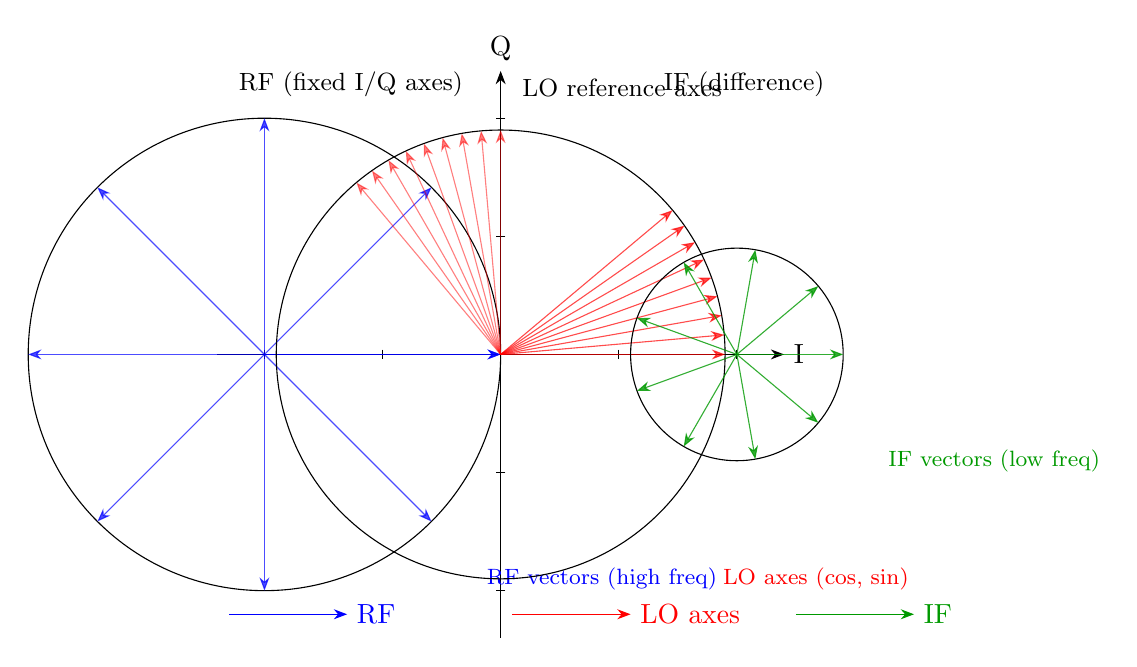
\begin{tikzpicture}[>=Stealth, scale=3]

% parameters
\def\n{8}             % number of sample arrows
\def\rfangle{0.0}     % initial angle for RF (deg)
\def\loangle{5.0}     % LO rotates a bit slower (deg per sample)
\def\ifangle{ }       % computed as rf - lo
\def\radiusRF{1.0}
\def\radiusLO{0.95}
\def\radiusIF{0.45}

% Draw axes (fixed IQ)
\draw[->] (-1.2,0) -- (1.2,0) node[right] {I};
\draw[->] (0,-1.2) -- (0,1.2) node[above] {Q};
\foreach \x in {-1,-0.5,0.5,1} \draw (\x,0.02) -- (\x,-0.02);
\foreach \y in {-1,-0.5,0.5,1} \draw (0.02,\y) -- (-0.02,\y);

% Title labels
\node[anchor=south west] at (-1.15,1.05) {\small RF (fixed I/Q axes)};
\node[anchor=south west] at (0.05,1.05) {\small LO reference axes};
\node[anchor=south west] at (0.65,1.05) {\small IF (difference)};

% Draw three regions: left (RF), middle (LO axes), right (IF)
% We will place each region by translating coordinates.

% --- RF region (translated left) ---
\begin{scope}[xshift=-1.0cm]
  % unit circle
  \draw[thin] (0,0) circle (\radiusRF);
  % draw sampled RF arrows (fast rotation)
  \foreach \k in {0,...,\n}{
    \pgfmathsetmacro{\ang}{\rfangle + 360*\k/\n} % simulate rotation
    \draw[blue,->,opacity=0.7] (0,0) -- ({\radiusRF*cos(\ang)},{\radiusRF*sin(\ang)});
  }
  \node[blue,right] at (0.9, -0.95) {\footnotesize RF vectors (high freq)};
\end{scope}

% --- LO region (center) ---
\begin{scope}[xshift=0.0cm]
  % circular axes showing LO as rotating basis vectors
  \draw[thin] (0,0) circle (\radiusLO);
  % draw LO basis arrows (cos,sin) at sample times
  \foreach \k in {0,...,\n}{
    \pgfmathsetmacro{\anglo}{\loangle * \k}
    % show the LO basis vector (cos)
    \draw[red,->,opacity=0.7] (0,0) -- ({\radiusLO*cos(\anglo)},{\radiusLO*sin(\anglo)});
    % show the LO quadrature (sin) as perpendicular
    \draw[red,->,opacity=0.5] (0,0) -- ({\radiusLO*cos(\anglo+90)},{\radiusLO*sin(\anglo+90)});
  }
  \node[red,right] at (0.9, -0.95) {\footnotesize LO axes (cos, sin)};
\end{scope}

% --- IF region (translated right) ---
\begin{scope}[xshift=1.0cm]
  \draw[thin] (0,0) circle (\radiusIF);
  % IF vectors = RF angle - LO angle (slow rotation)
  \foreach \k in {0,...,\n}{
    \pgfmathsetmacro{\angrf}{\rfangle + 360*\k/\n}
    \pgfmathsetmacro{\anglo}{\loangle * \k}
    \pgfmathsetmacro{\angif}{\angrf - \anglo}
    \draw[green!60!black,->,opacity=0.8] (0,0) -- ({\radiusIF*cos(\angif)},{\radiusIF*sin(\angif)});
  }
  \node[green!60!black,right] at (0.6, -0.45) {\footnotesize IF vectors (low freq)};
\end{scope}

% small legend
\begin{scope}[xshift= -1.15cm, yshift=-1.1cm]
  \draw[blue,->] (0,0) -- (0.5,0) node[right]{ RF};
  \draw[red,->] (1.2,0) -- (1.7,0) node[right]{ LO axes};
  \draw[green!60!black,->] (2.4,0) -- (2.9,0) node[right]{ IF};
\end{scope}

\end{tikzpicture}

\end{document}